\chapter [Introdução]{Introdução}

\section{Contextualização}

% Falar sobre a importância das energias renováveis no contexto mundial

A crescente demanda de energia e a urgente atenção para causas ambientais exigem sistemas de energia eficientes e ecológicos. 
As energias renováveis são consideradas como alternativas promissoras para os sistemas convencionais de combustíveis fósseis, adotados em peso ao redor do mundo, e portanto, tem chamado cada vez mais atenção \cite{Guo2018}.
A Fig. \ref{fig:energy-resources} mostra o potencial que as energias renováveis tem de fornecer até mais de 3000 vezes a demanda atual de energia.

\begin{figure}[!hbt]
	\begin{center}
    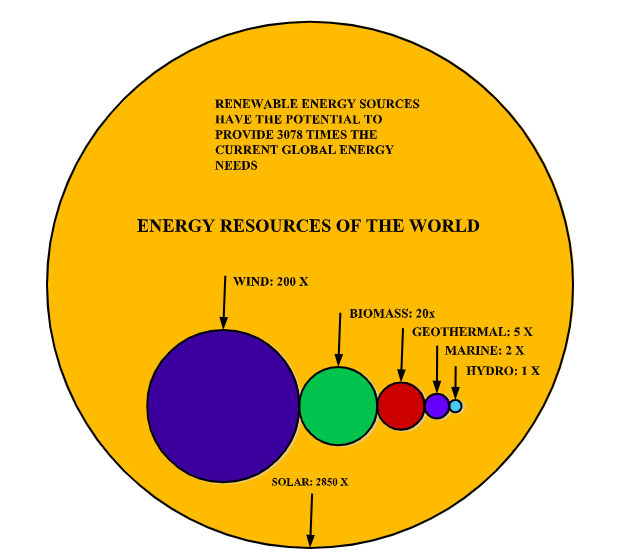
\includegraphics[width=0.5\textwidth]{figuras/Energy_Resources_of_The_World.png}
    \caption{Recursos de energia no mundo. Fonte: \cite{Ellabban2014}}
    \label{fig:energy-resources}
    \end{center}
\end{figure}

Uma análise baseada em cenários realizada pela Perspectiva Mundial de Energia (do inglês \textit{WEO - World Energy Outlook}) da Agência Internacional de Energia (\textit{IEA - International Energy Agency}) descreve que diferentes futuros possíveis podem ser atingidos para o sistema de energia no que tange combustíveis e tecnologias.
Há um constraste com diferentes caminhos, baseados nas políticas atuais e nas planejadas, sobre aquelas que de fato podem atingir as metas climáticas de longo prazo sob o Acordo de Paris, reduzir a poluição do ar e garantir o acesso universal à energia. 

Em todos os casos, os governos terão uma influência crítica na direção do futuro sistema energético. 
De acordo com as políticas atuais e planejadas, modeladas no \textbf{Cenário de Novas Políticas}, a demanda mundial de energia deve crescer mais de 25\% até 2040, exigindo mais de US\$ 2 trilhões por ano de investimento em novos suprimentos de energia \cite{WEO2018}.

As energias renováveis tiveram um forte crescimento nos últimos anos, com o setor de energia elétrica na liderança e quebrando recordes de níveis de investimento e implantação.
Mas a adoção de fontes renováveis tem sido mais lenta na indústria, nos edifícios e nos transportes.
Algumas tecnologias de energias renováveis, como a energia solar fotovoltaica e a eólica \textit{onshore}, estão adquirindo competitividade; outras, como a energia eólica \textit{offshore}, estão equilibradas entre a necessidade de apoio e a competitividade, enquanto tecnologias como a energia das marés e ondas ainda precisam de suporte.

A Fig. \ref{fig:geracao-capacidade-energias-renovaveis} mostra uma prospecção da geração e capacidade das energias renováveis ao redor do mundo. 
No \textbf{Cenário de Novas Políticas}, a geração de eletricidade a partir de fontes renováveis quase triplica até 2040 e representa mais de 40\% da geração geral.
Há um crescimento no uso direto de fontes renováveis em aplicações de transporte e aquecimento, mas a participação destes setores é menor.
A participação das energias renováveis no aquecimento de casas e edifícios aumenta neste cenário em cinco pontos percentuais, para 15 \% em 2040.
Espera-se que cerca de 60\% desse aumento ocorra na China, União Europeia, Índia e Estados Unidos, que são hoje maiores consumidores de sistemas de calefação à base de energias renováveis.
Nos transportes, a parcela de energias renováveis diretas e indiretas mais que dobra, atingindo cerca de 8\%. 
Prevê-se que a demanda por biocombustíveis aumente para 4,7 mboe/d, representando 6\% do uso de energias renováveis no transporte em 2040 \cite{WEO2018}.

\begin{figure}[!hbt]
	\begin{center}
    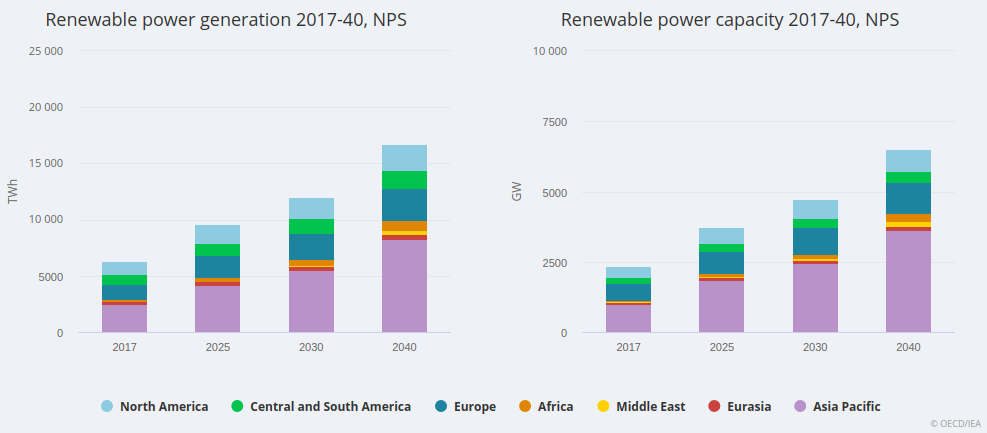
\includegraphics[width=\textwidth]{figuras/geracao_capacidade_potencia_energias_renovaveis.png}
    \caption{Prospecção da geração de energia e capacidade de potência com a utilização de energias renováveis de 2017 à 2040. Fonte: \cite{WEO2018}}
    \label{fig:geracao-capacidade-energias-renovaveis}
    \end{center}
\end{figure}

As mudanças climáticas e a poluição do ar local estão entre os principais fatores para a transição energética no mundo. 
A poluição do ar local é o principal fator em países como China e Índia. 
Na Europa, há uma atenção crescente aos efeitos nocivos à saúde da poluição atmosférica, amplamente relacionados ao fornecimento e uso de energia \cite{Gielen2019}.

% Falar sobre a utilizacao, crescimento e perspectivas da utilização da energia eólica no contexto mundial

Nos últimos 30 anos, os sistemas envolvendo energia solar e eólica tem melhorado suas características de desempenho e experimentado um rápido crescimento de vendas. 
De fato, a energia eólica parece ter uma vantagem maior, pois esta já está pronta para ser emprega em larga escala a um custo razoável, ainda que em comparação com outras fontes \cite{Kumar2016}.

Segundo a Associação Internacional de Energia Eólica (WWEA - \textit{World Wind Energy Association}), a capacidade mundial de potência usando energia eólica atingiu 597 GW, com um adição de 50,1 GW em 2018.
O ano de 2018 foi o segundo ano consecutivo com um número crescente de novas instalações, porém com uma taxa mais baixa de 9,1\%, em comparação com 2017, que experimentou uma taxa de 10,8\%.
Todas as turbinas eólicas instaladas até o final de 2018 podem cobrir até cerca de 6\% da demanda global de eletricidade.

A Tab. \ref{tab:capacidade-instalada} mostra um comparativo da capacidade instalada de unidades eólicas entre os anos de 2015 e 2018 entre vários países.
Verifica-se que os maiores líderes de mercado são a China e os EUA, tendo o Brasil um papel de destaque no comparativo mundial \cite{WEI}.

\begin{table}[h]
	\centering
	\caption{Capacidade das instalações eólicas até o final de 2018 (MW). Fonte: \cite{WEI}}
	\label{tab:capacidade-instalada}
	
	\begin{tabular}{ccccc}
		\toprule
		\textbf{País/Região} & \textbf{2018} & \textbf{2017} & \textbf{2016} & \textbf{2015}\\
		\midrule
		China & 216870 & 195730 & 168730 & 148000 \\
		Estados Unidos & 96363 & 88775 & 82033 & 73867 \\
		Alemanha & 59313 & 56190 & 50019 & 45192 \\
		Índia & 35017 & 32879 & 28279 & 24759 \\
		Espanha & 23494 & 23026 & 23020 & 22987 \\
		Reino Unido & 20743 & 17852 & 14512 & 13614 \\
		França & 15313 & 13760 & 12065 & 10293 \\
        Brasil & 14490 & 12763 & 10800 & 8715 \\
        Canadá & 12816 & 12239 & 11898 & 11205 \\
        Resto do mundo & 102138 & 93173 & 85582 & 76653 \\
        \textbf{Total geral} & \textbf{596556} & \textbf{546388} & \textbf{486939} & \textbf{435284} \\
		\bottomrule
	\end{tabular}
\end{table}

% Comentar sobre a matriz energética atual brasileira

A energia éolica tem tido papel de importância no Brasil e seu crescimento tem sido rápido. 
Segundo \cite{Pinto2019}, a indústria eólica vem crescendo a uma taxa média anual de 2,3 GW, o que em termos de geração eólica total, levou o país a atingir cerca de 21,626 GWh em 2015.

O Brasil, por conta de sua extensão territorial e por possuir extensas planícies e relevos, 
assim como climas que se diversificam entre quentes e úmidos que colaboram para a ocorrência de ventos fortes 
- velocidades médias anuais de até 8,5 m/s em estados do Nordeste e acima de 7 m/s no Rio Grande do Sul - 
regulares e de grande estabilidade em sua direção, tem um potencial eólio-elétrico estimado, pelo Atlas do Potencial Eólico Brasileiro, em 143 GW \cite{Pinto2019}.

A Fig. \ref{fig:matriz-energetica-brasileira} apresenta a matriz energética brasileira e mostra que a energia eólica já é a segunda maior fonte de energia elétrica da matriz. 
De fato, no final de 2017, a participação das eólicas era de 8,1 \%, saltando para 9,0 \% em 2019, mostrando o crescimento e a relevância desta fonte de energia no âmbito nacional \cite{ABEeolica}.

% Falar sobre a utilização, crescimento e perspectivas da utilização da energia eólica no cenário brasileiro

\begin{figure}[!hbt]
	\begin{center}
    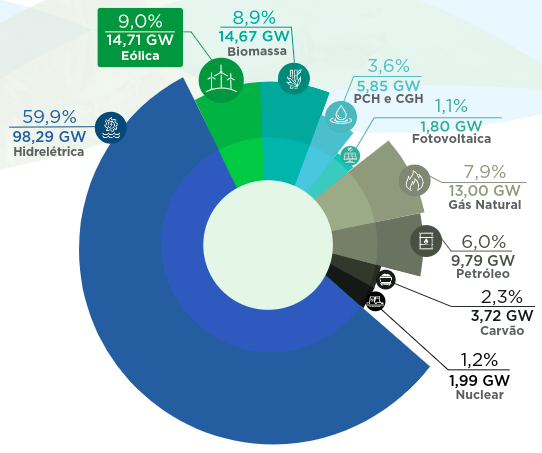
\includegraphics[width=0.5\textwidth]{figuras/matriz_eletrica_brasileira.png}
    \caption{Matriz Energética Brasileira (GW). Fonte: \cite{ABEeolica}}
    \label{fig:matriz-energetica-brasileira}
    \end{center}
\end{figure}

\section{Descrição do Problema}

% Comentar sobre as normas e regulamentos que regem a utilização da energia eólica no mundo e no Brasil
% Comentar sobre a utilização e projetos de conversores eletrônicos de potência
% Fazer um parágrafo relacionionando o projeto de conversores eletrônicos com a proposta apresentada no presente trabalho

\section{Objetivos}

\section{Organização do Trabalho}


